\chapter{Appendix 15}
\label{a:appendix}

\section{Algorithm Pseudocodes}
\begin{figure}[h]
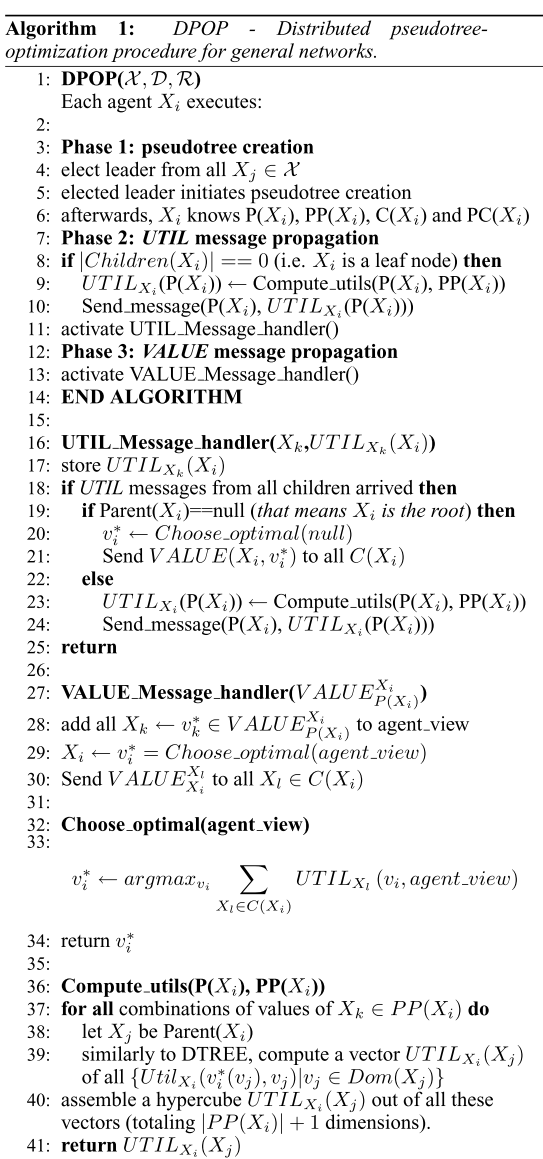
\includegraphics[width=200px]{graphics/dpop_ps}
\centering
\caption{The Pseudocode of DPOP}
\label{fig:dpopps}
\end{figure}
\begin{figure}[h]
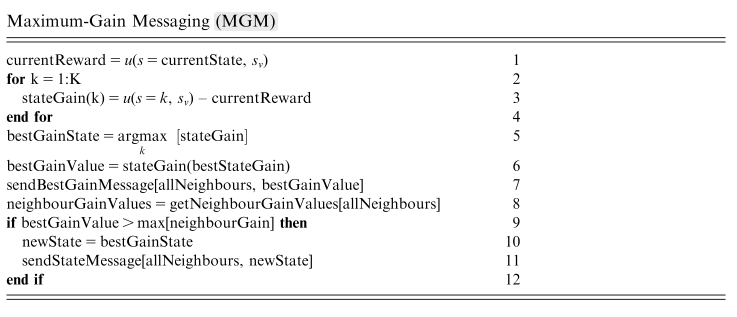
\includegraphics[width=300px]{graphics/mgm_ps}
\centering
\caption{The Pseudocode of MGM}
\label{fig:mgmps}
\end{figure}
\begin{figure}[h]
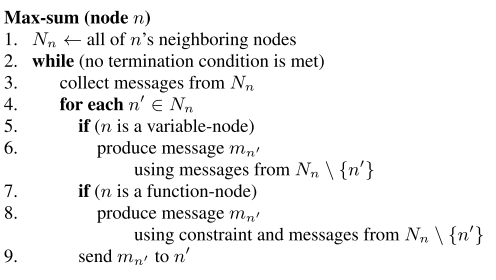
\includegraphics[width=300px]{graphics/maxsum_ps}
\centering
\caption{The Pseudocode of MaxSum}
\label{fig:maxsumps}
\end{figure}

\section{Results I: Additional Data}

\begin{figure}[h]
\centering
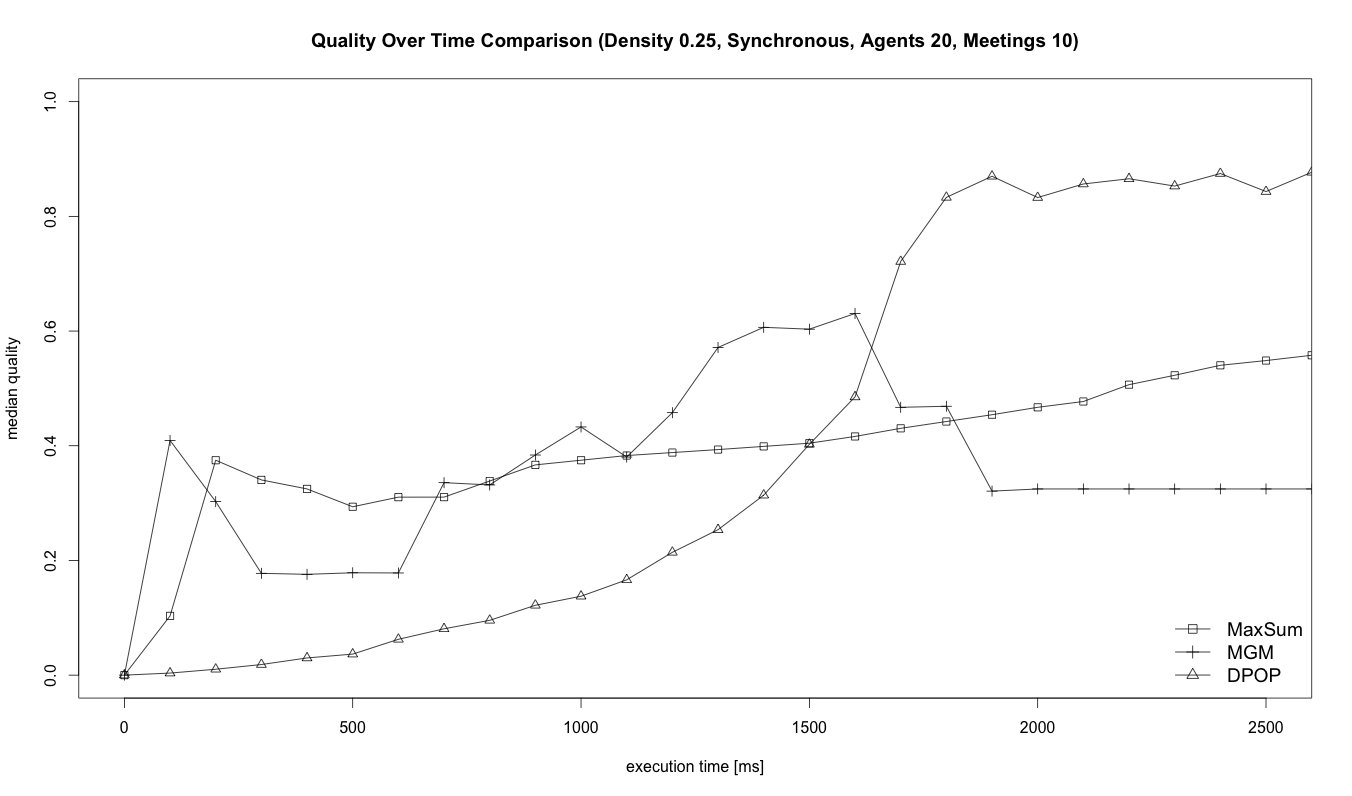
\includegraphics[width=430px]{graphics/experiments/static/st_2}
\caption{20/10, 0.25 density, all three, utility}
\label{fig:st_2}
\end{figure}

\begin{figure}[h]
\centering
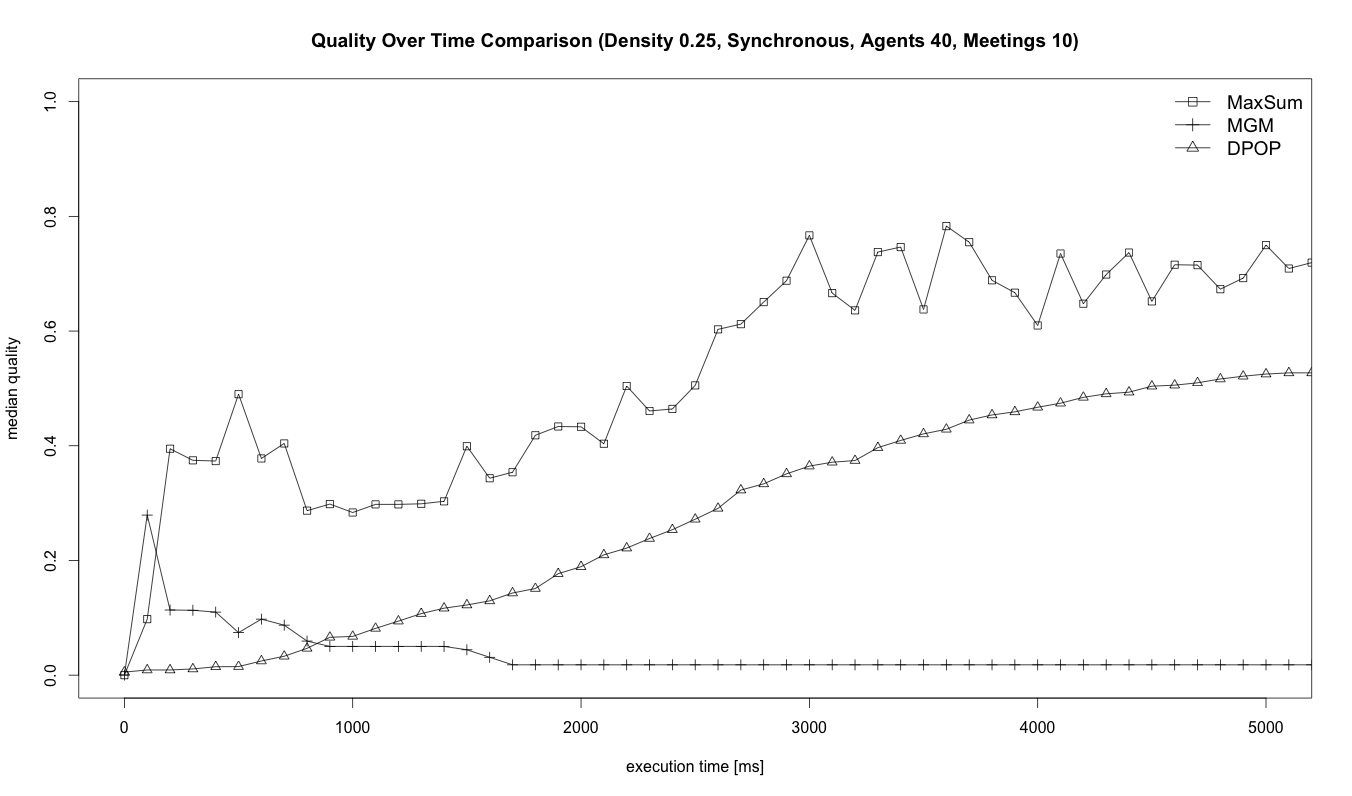
\includegraphics[width=430px]{graphics/experiments/static/st_4}
\caption{20/10, 0.25 density, all three, utility}
\label{fig:st_3}
\end{figure}

\section{Results II: Additional Data}

\begin{figure}[h]
\centering
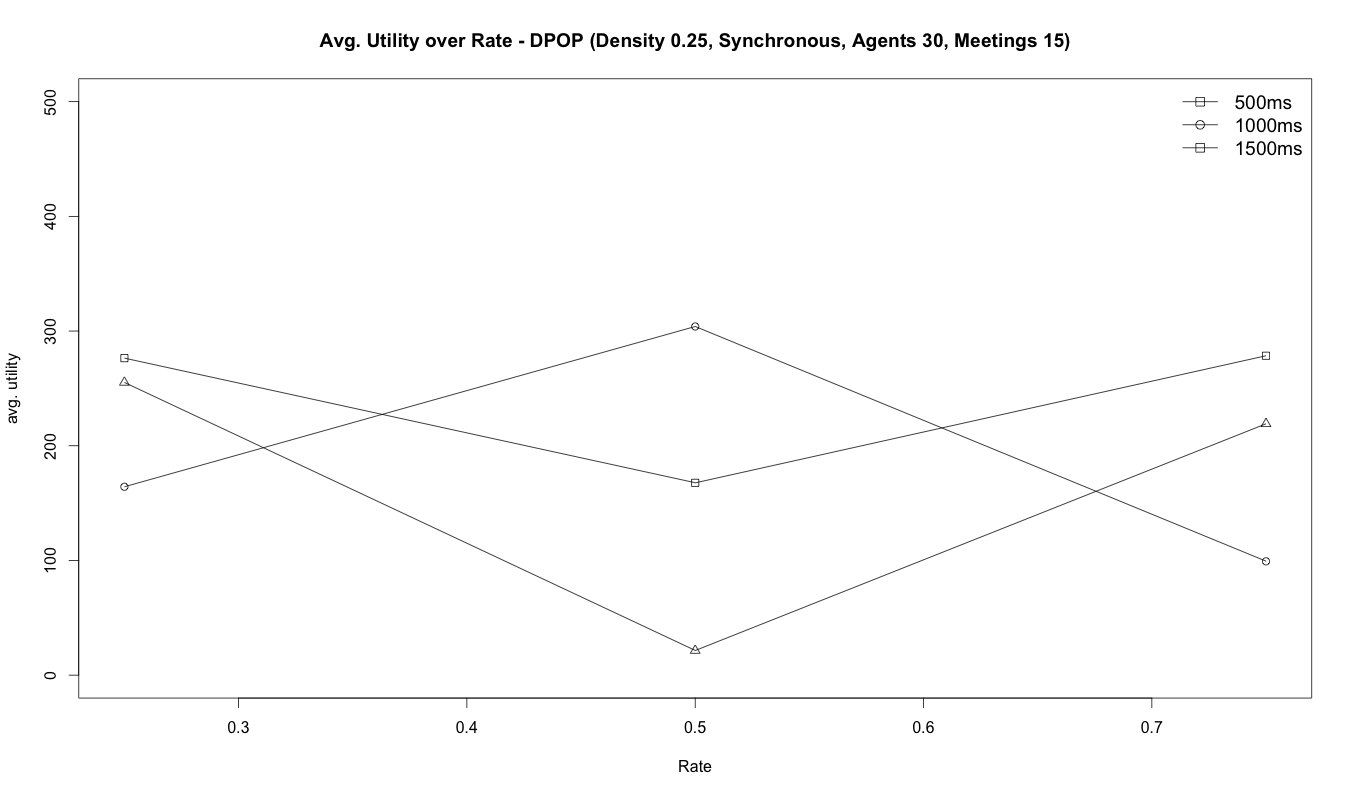
\includegraphics[width=430px]{graphics/experiments/dynamic/d_6}
\caption{20/10, 0.25 density, all three, utility}
\label{fig:d_6}
\end{figure}